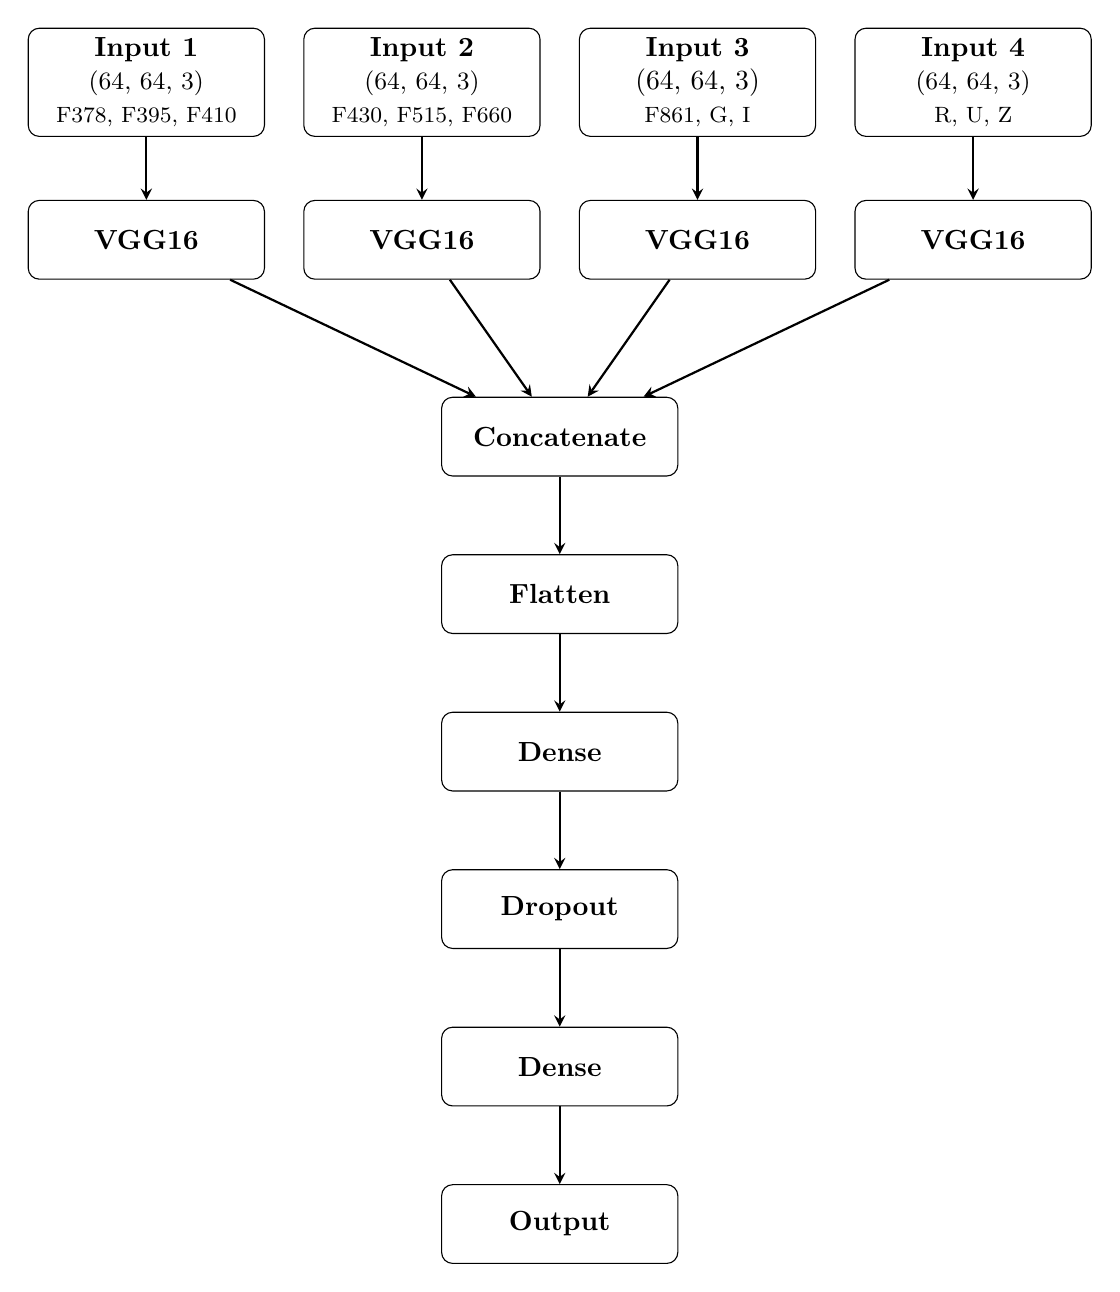
\begin{tikzpicture}
  \tikzstyle{basenode} = [rectangle, rounded corners, minimum width=3cm, minimum height=1cm,text centered, draw=black, align=center]
  \tikzstyle{arrow} = [thick,->,>=stealth]

  \node (inp1) [basenode]
  {{\bf Input 1}\\{\small (64, 64, 3)}\\{\footnotesize F378, F395, F410}};
  \node (inp2) [basenode, right of=inp1, xshift=2.5cm]
  {{\bf Input 2}\\{\small (64, 64, 3)}\\{\footnotesize F430, F515, F660}};
  \node (inp3) [basenode, right of=inp2, xshift=2.5cm]
  {{\bf Input 3}\\(64, 64, 3)\\{\footnotesize F861, G, I}};
  \node (inp4) [basenode, right of=inp3, xshift=2.5cm]
  {{\bf Input 4}\\{\small (64, 64, 3)}\\{\footnotesize R, U, Z}};
  \node (vgg1) [basenode, below of=inp1, yshift=-1cm] {{\bf VGG16}};
  \node (vgg2) [basenode, below of=inp2, yshift=-1cm] {{\bf VGG16}};
  \node (vgg3) [basenode, below of=inp3, yshift=-1cm] {{\bf VGG16}};
  \node (vgg4) [basenode, below of=inp4, yshift=-1cm] {{\bf VGG16}};
  \node (concatenate) [basenode, below of=vgg2, xshift=1.75cm, yshift=-1.5cm]
  {{\bf Concatenate}};
  \node (flatten) [basenode, below of=concatenate, yshift=-1cm] {{\bf Flatten}};
  \node (dense1) [basenode, below of=flatten, yshift=-1cm] {{\bf Dense}};
  \node (dropout1) [basenode, below of=dense1, yshift=-1cm] {{\bf Dropout}};
  \node (dense2) [basenode, below of=dropout1, yshift=-1cm] {{\bf Dense}};
  \node (out) [basenode, below of=dense2, yshift=-1cm] {{\bf Output}};

  \draw [arrow] (inp1) -- (vgg1);
  \draw [arrow] (inp2) -- (vgg2);
  \draw [arrow] (inp3) -- (vgg3);
  \draw [arrow] (inp4) -- (vgg4);
  \draw [arrow] (vgg1) -- (concatenate);
  \draw [arrow] (vgg2) -- (concatenate);
  \draw [arrow] (vgg3) -- (concatenate);
  \draw [arrow] (vgg4) -- (concatenate);
  \draw [arrow] (concatenate) -- (flatten);
  \draw [arrow] (flatten) -- (dense1);
  \draw [arrow] (dense1) -- (dropout1);
  \draw [arrow] (dropout1) -- (dense2);
  \draw [arrow] (dense2) -- (out);
\end{tikzpicture}